\documentclass[letter,12 pt,titlepage]{article}
 
\usepackage[utf8]{inputenc}
\usepackage[spanish]{babel}
\usepackage[T1]{fontenc}
\usepackage{lmodern}
\usepackage{amssymb}
\usepackage{parskip}
\usepackage{xcolor}
\usepackage{multicol}
\usepackage{anysize}
\usepackage{enumerate}
\usepackage{url}
\usepackage{pdfpages}
\usepackage[hidelinks]{hyperref}
\usepackage{chngcntr}
\counterwithout{footnote}{section}

%izq der arr ab
\marginsize{3 cm}{3 cm}{1.5 cm}{2.5 cm} 

\begin{document}
    \begin{titlepage}
        \centering
        
\includegraphics[width=0.15\textwidth]{img/escudo_fi_color.png}\par\vspace{1cm}
        {\scshape\LARGE Facultad de Ingeniería \par}
        \vspace{1cm}
        {\scshape\Large Estructura y Programación de Computadoras
        \par}
        \vspace{1cm}
        {\scshape\Large Grupo 2
        \par}
        \vspace{1.5cm}
        {\huge\bfseries Proyecto Nº1\par}
        \vspace{2cm}
        {\Large 
            Martínez Baeza José Alfonso
        \par}
        \vfill
        {\large 22 de abril de 2020\par}
    \end{titlepage}
    \newpage
    \tableofcontents
    \newpage

    \section{Introducción}

    \subsection{Descripción del problema}

        Se requiere elaborar un programa que realice operaciones básicas entre dos números ingreseados por el usuario y que muestre los resultados en pantalla.

    \subsection{Planteamiento del problema}

        Desarrollar un programa en lenguaje ensamblador para arquitectura Intel x86 que solicite ingresar 2 números desde el teclado, y que calcule:
        
        \begin{center}
            \begin{minipage}{0.95\linewidth}
                \begin{itemize}
                    \item La suma de ambos números.
                    \item La resta del primer número menos el segundo.
                    \item La multiplicación de ambos números.
                    \item El cociente de la división del primer número entre el segundo.
                    \item El residuo de la división del primer número entre el segundo.
                \end{itemize}
            \end{minipage}
        \end{center}

        \textbf{Consideraciones:}
        \begin{center}
            \begin{minipage}{0.95\linewidth}
                \begin{itemize}
                    \item Los números deben estar en sistema decimal (dígitos de 0-9).
                    \item Los números deberán ser enteros sin signo.
                    \item Cada número introducido por el usuario puede ser de hasta 4 dígitos. El programa debe restringir que el usuario introduzca más números.
                    \item Al ingresar los números, no deberá aceptar caracteres que no sean numéricos.
                \end{itemize}
            \end{minipage}
        \end{center}

    \section{Desarrollo}

    Para la realización de este proyecto nos apoyaremos del uso de macros y procedimientos dentro del lenguaje ensamblador para poder reducir el número de líneas de código, también se hará uso de saltos condicionales, variables auxiliares, etc.

    \subsection{Macros}

    Se programaron dos macros en este proyecto: \textit{clear} y \textit{delete} para limpiar la pantalla y eliminar un caracter respectivamente.

    \subsubsection{Clear}

    Esta macro hace uso de la interrupción $10h$ \footnote{\url{http://ict.udlap.mx/people/oleg/docencia/Assembler/asm_interrup_10.html}}, junto con el valor $00h$ selecciona y activa el modo de vídeo especificado y se borra la pantalla.

    \begin{verbatim}
clear macro        ; macro para limpiar pantalla
    mov ah,0h      ;AH = 0
    mov al,3h      ;AL = 3h
    int 10h        ;Interrupcion 10h
endm clear
    \end{verbatim}

    \subsubsection{Delete}
    \subsubsection{Imprimir Digito}
    \subsection{Procedimientos}
    \subsubsection{Leer Número}
    Para leer un número en lenguaje ensamblador, es necesario leer cada dígito por separado. Para el usuario da la impresión de ingresar el número completo.

    Para esto se hizo uso del valor $08h$ guardado en el registro $AH$ para que la interrupción $21h$ nos permita leer datos sin mostrarlos en pantalla; en caso de  que el valor en el registro $AL$ corresponda a un número en su respectivo código ASCII \footnote{\url{https://ascii.cl/es/}}, $i.e.$ entre $30h$ y $39h$, entonces se dibujará en pantalla, de lo contrario seguirá leyendo dígitos. El planteamiento se observa de la siguiente manera:

    \begin{verbatim}
...
leer:
  mov ah,08h   ; Instrucción para ingresar datos sin verlos en pantalla
  int 21h      ; Interrupcion 21h para controlar funciones del S.O.

  cmp al,40h   ; Compara AL con 40h
  jae leer     ; Si es mayor o igual a 40h vuelve a leer
  cmp al,30h   ; Compara AL con 30h
  jb leer      ; Si es menor a 30h vuelve a leer

  mov ah,02h   ; AH = 02H, prepara AH para imprimir un caracter
  mov dl,al    ; DL = AL, AL contiene el caracter a imprimir
  int 21h      ; Interrupcion 21h para controlar funciones del S.O.
...
    \end{verbatim}
    
    Una vez que se consiguió leer los dígitos es necesario programar un bloque de código que nos permita hacer la espera de un `enter' para continuar, a su vez, también se requiere que se haya ingresado por lo menos un dígito para continuar, por esto se implementó un contador guardado en el registro CL y es así como el código anterior se complementó de la siguiente manera:

    \begin{verbatim}
...
  cl = 0
leer:
  mov ah,08h     ; Instrucción para ingresar datos sin verlos en pantalla
  int 21h        ; Interrupcion 21h para controlar funciones del S.O.

  cmp cl,0       ; Compara cl con 0
  je sinNumero   ; Si CL == 0, salta a la etiqueta sinNumero para obligar 
                 ; al usuario a ingresar por lo menos un digito

  cmp al,0Dh     ; Compara AL con el valor hexadecimal del 'enter'
  jne sinNumero  ; Si el usuario da 'enter'
  jmp flujo2

sinNumero:
  cmp al,40h     ; Compara AL con 40h
  jae leer       ; Si es mayor o igual a 40h vuelve a leer
  cmp al,30h     ; Compara AL con 30h
  jb leer        ; Si es menor a 30h vuelve a leer

  mov ah,02h     ; AH = 02H, prepara AH para imprimir un caracter
  mov dl,al      ; DL = AL, AL contiene el caracter a imprimir
  int 21h        ; Interrupcion 21h para controlar funciones del S.O.

flujo2:
...
    \end{verbatim}

    Al ser números de cuatro dígitos, el registro CL nos ayudará a controlar la cantidad de dígitos que el usuario puede ingresar, pues este condiciona al programa a que mientras CL sea menor a 4 entonces el usuario puede seguir ingresando dígitos.

    Como cada dígito es ingresado por separado, es necesario multiplicarlo por el valor correspondiente a la posición que ocupa en el número completo y guardarlos en variables auxiliares para posteriormente sumarlos, $i.e.$, unidades, decenas, centenas o unidades de millar.

    Dependiendo del valor de CL ($0, 1, 2$ o $3$) el código se implementa de la siguiente manera:

    \begin{verbatim}
...
    cmp cl,0       ; Compara cl con 0
    je miles       ; Si CL == 0 es porque es el primer digito

    cmp cl,1       ; Compara CL con 1
    je centenas    ; Si CL == 1 es porque es el segundo digito

    cmp cl,2       ; Compara cl con 2
    je decenas     ; Si CL == 2 es porque es el tercer digito

    cmp cl,3       ; Compara cl con 3
    je unidades    ; Si CL == 3 es porque es el cuarto digito

miles:
    sub al,30h     ; Resta 30h para obtener el valor numerico 
                   ; del codigo ascii
    mov um,al      ; um = AL
    jmp flujo1     ; salta al flujo 1

centenas:
    sub al,30h     ; Resta 30h para obtener el valor numerico 
                   ; del codigo ascii
    mov c,al       ; c = AL
    jmp flujo1     ; salta al flujo 1

decenas:
    sub al,30h     ; Resta 30h para obtener el valor numerico 
                   ; del codigo ascii
    mov d,al       ; d = AL
    jmp flujo1     ; salta al flujo 1

unidades:
    sub al,30h     ; Resta 30h para obtener el valor numerico 
                   ; del codigo ascii
    mov u,al       ; u = AL

flujo1:
    add cl,1       ; CL = CL + 1
    cmp cl,4       ; Compara CL con 4
    jb leer        ; Si CL < 4 entonces lee el siguiente dígito

flujo2:
    xor ah,ah      ; limpia la parte alta del registro AX
    mov al,um      ; AL = um
    mov bx,1000    ; BX = 1000
    mul bx         ; DX:AX = AX * BX
    mov num1,ax    ; num = AX

    xor ah,ah      ; limpia la parte alta del registro AX
    mov al,c       ; AL = c
    mov bl,100     ; BL = 100
    mul bl         ; AX = AL * BL
    add num1,ax    ; num1 = num1 + AX

    xor ah,ah      ; limpia la parte alta del registro AX
    mov al,d       ; AL = d
    mov bl,10      ; BL = 10
    mul bl         ; AX = AL * BL
    add num1,ax    ; num1 = num1 + AX

    xor ah,ah      ; limpia la parte alta del registro AX
    mov al,u       ; AL = u
    add num1,ax    ; num1 = num1 + AX
...
    \end{verbatim}

    En este punto el programa ya nos permite varias cosas:
    \begin{itemize}
        \item Leer únicamente caracteres numéricos.
        \item Leer un número de 4 dígitos como máximo.
        \item No permitir dar `enter' sin haber ingresado por lo menos un dígito.
        \item Dejar de leer dígitos al dar enter.
    \end{itemize}

    Sin embargo, nos podemos dar cuenta de que al romper el ciclo de lectura al dar `enter', los números van a multiplicarse de la misma manera independientemente de la cantidad de dígitos ingresados. Por ejemplo, al ingresar el número $123$ el programa realizará las siguientes operaciones:

    \begin{center}
    \begin{minipage}{0.3\linewidth}
        \begin{flushright}
        $um = 1 * 1000 = 1000$\\
        $ c = 2 *  100 =  200$\\
        $ d = 3 *   10 =   30$\\
        $ u = 0 $
        \end{flushright}
    \end{minipage}
    \end{center}

    Al sumarlos obtendremos el número 1230, es decir, un número distinto a 123. No obstante podemos notar que al dividir entre 10 llegamos al número que necesitamos.

    Veamos otro ejemplo con el número 93:

    \begin{center}
    \begin{minipage}{0.3\linewidth}
        \begin{flushright}
        $um = 9 * 1000 = 9000$\\
        $ c = 3 *  100 =  300$\\
        $ d = 0 *   10 =   0$\\
        $ u = 0 $
        \end{flushright}
    \end{minipage}
    \end{center}

    En este caso obtenemos el número 9300, que al dividir entre 100, nuevamente llegamos al número correcto. De esta manera se implementó la solución comparando el valor de CL al momento de salir del ciclo de lectura de dígitos y dependiendo de eso se divide entre $1000,100$ o $10$.

    Es así como el código se complementó con lo siguiente:

    \begin{verbatim}
...
    cmp cl,1       ; Compara CL con 1
    je i1          ; Si Cl == 1 entonces salta a i1
    cmp cl,2       ; Compara CL con 2
    je i2          ; Si Cl == 2 entonces salta a i2
    cmp cl,3       ; Compara CL con 3
    je i3          ; Si Cl == 3 entonces salta a i3
    cmp cl,4       ; Compara CL con 4
    je flujo3      ; Si Cl == 4 entonces salta a flujo3  

i1:
    mov ax,num1    ; AX = num1
    mov bx,1000    ; BX = 1000
    div bx         ; DX:AX = AX / BX
    mov num1,ax    ; num = AX
    jmp flujo3     ; Salta a flujo3  
i2:
    mov ax,num1    ; AX = num1
    mov bx,100     ; BX = 100
    div bx         ; DX:AX = AX / BX
    mov num1,ax    ; num = AX
    jmp flujo3     ; Salta a flujo3  
i3:
    mov ax,num1    ; AX = num1
    mov bx,10      ; BX = 10
    div bx         ; DX:AX = AX / BX
    mov num1,ax    ; num = AX
    jmp flujo3     ; Salta a flujo3  

ingrese2:
...
    \end{verbatim}
    \subsubsection{Imprimir Número}
    \subsection{Suma}
    \subsection{Resta}
    \subsection{Multiplicación}
    \subsection{División}


    \section{Diagrama de Flujo.}

    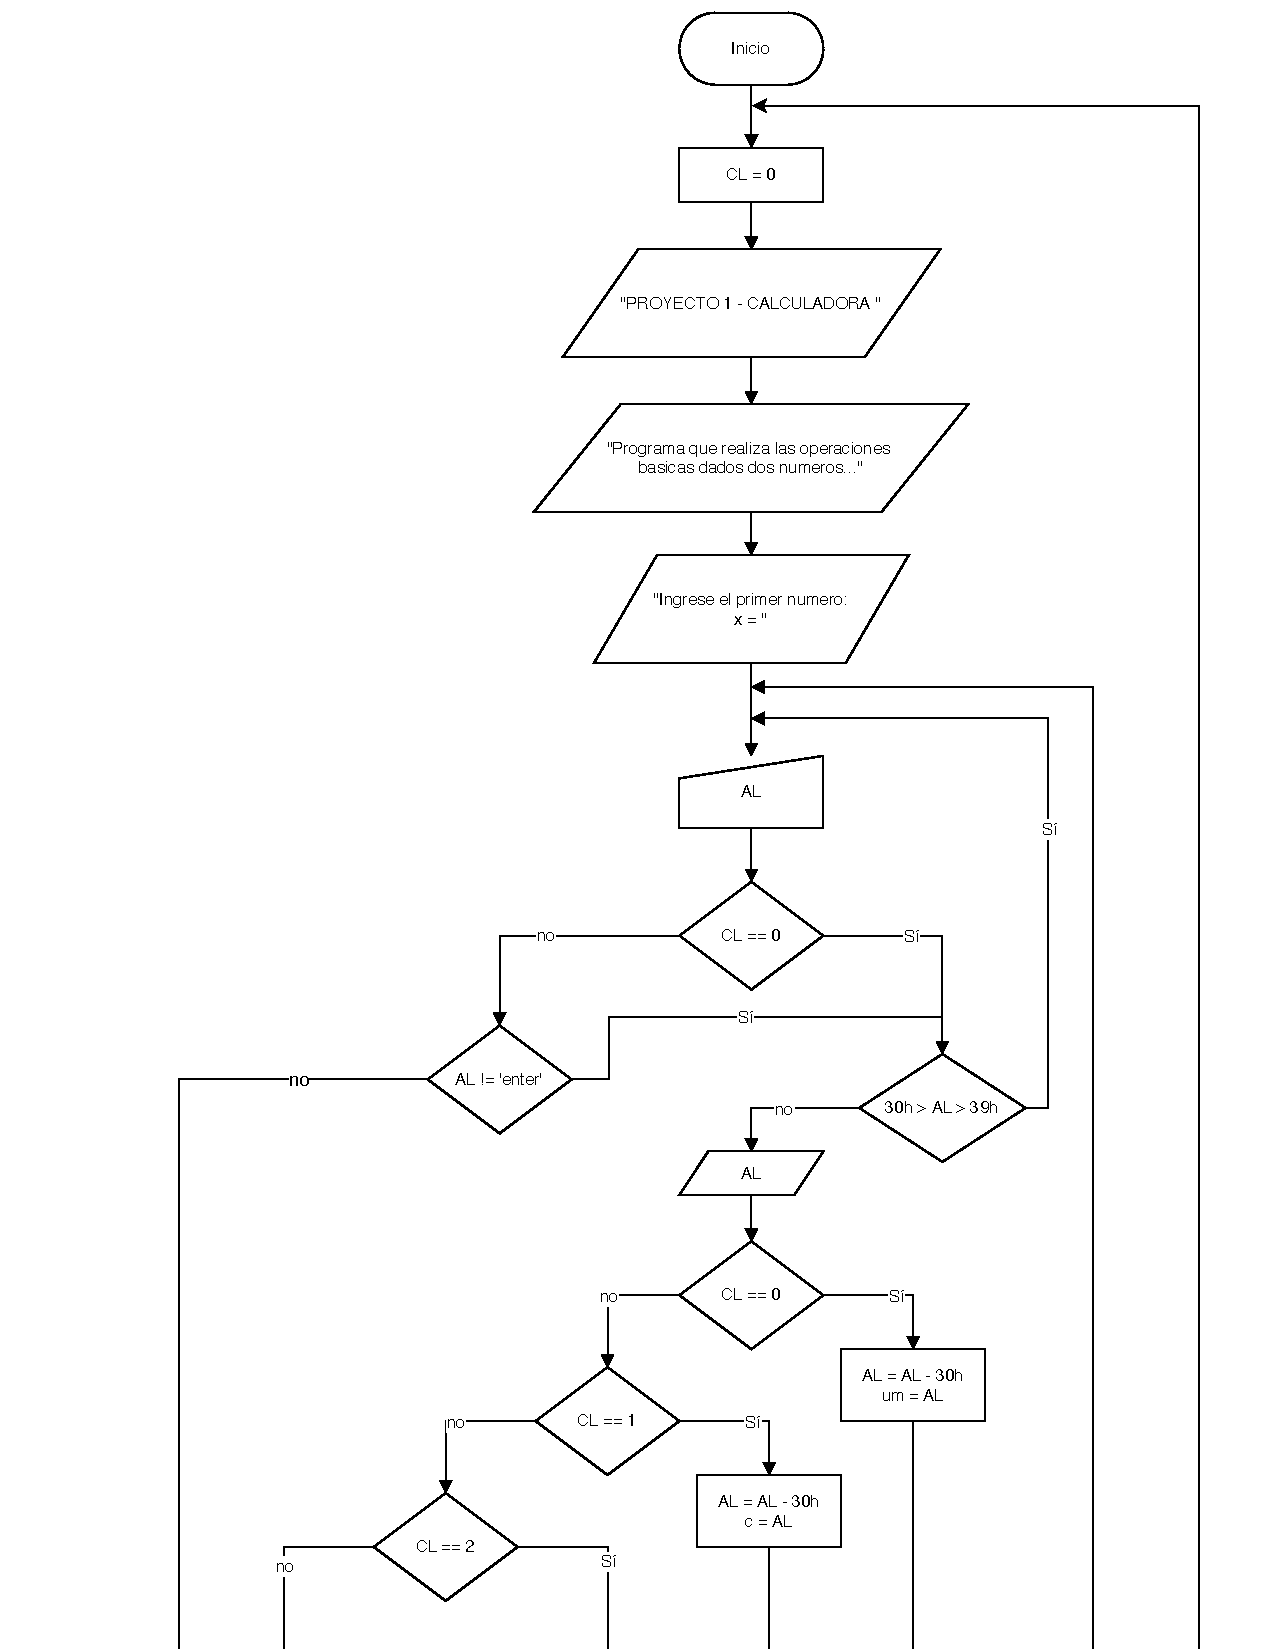
\includepdf[fitpaper=true, pages=1-14]{img/DF}

    \section{Conclusion}

    

\end{document}





